\chapter{Evaluation}
\label{chap:evaluation}
\begin{chapterintro}
In this chapter we will evaluate the game application through the information retrieved after its deployment
\end{chapterintro}

\cleardoublepage
\section{Overview}
In the following sections we will observe the impact that our application has taken after its deployment. We will analyze both Android and iOs application that we have deployed to Google Play and Apple Store respectively.

The metrics used in this chapter have been recovered using \textit{Game Analytics}. Although ideally we should have used Flurry to retrieved the desired metrics to write this chapter, the client restricted Flurry panel access two years after the application deployment.

Game Analytics is a free and powerful analytics tool for game developers, that helps us to understand player behavior and build better games.~\cite{gametrics1} It is natively included within Unity so we are able to access to lots of metrics out of the box.

\section{Acquisition}

In this section we are going to revise the user acquisition. The most important metrics for user acquisition are number and location of installations. These two metrics are by far the easiest way to tell if our application is something that people find valuable.

We have to notice that although our application is free to download, the pack with the physical instrument pieces should be bought in the client physical stores. This physical pack is shown in Figure \ref{fig:instruments-pack}

\begin{figure}[h]
\centering
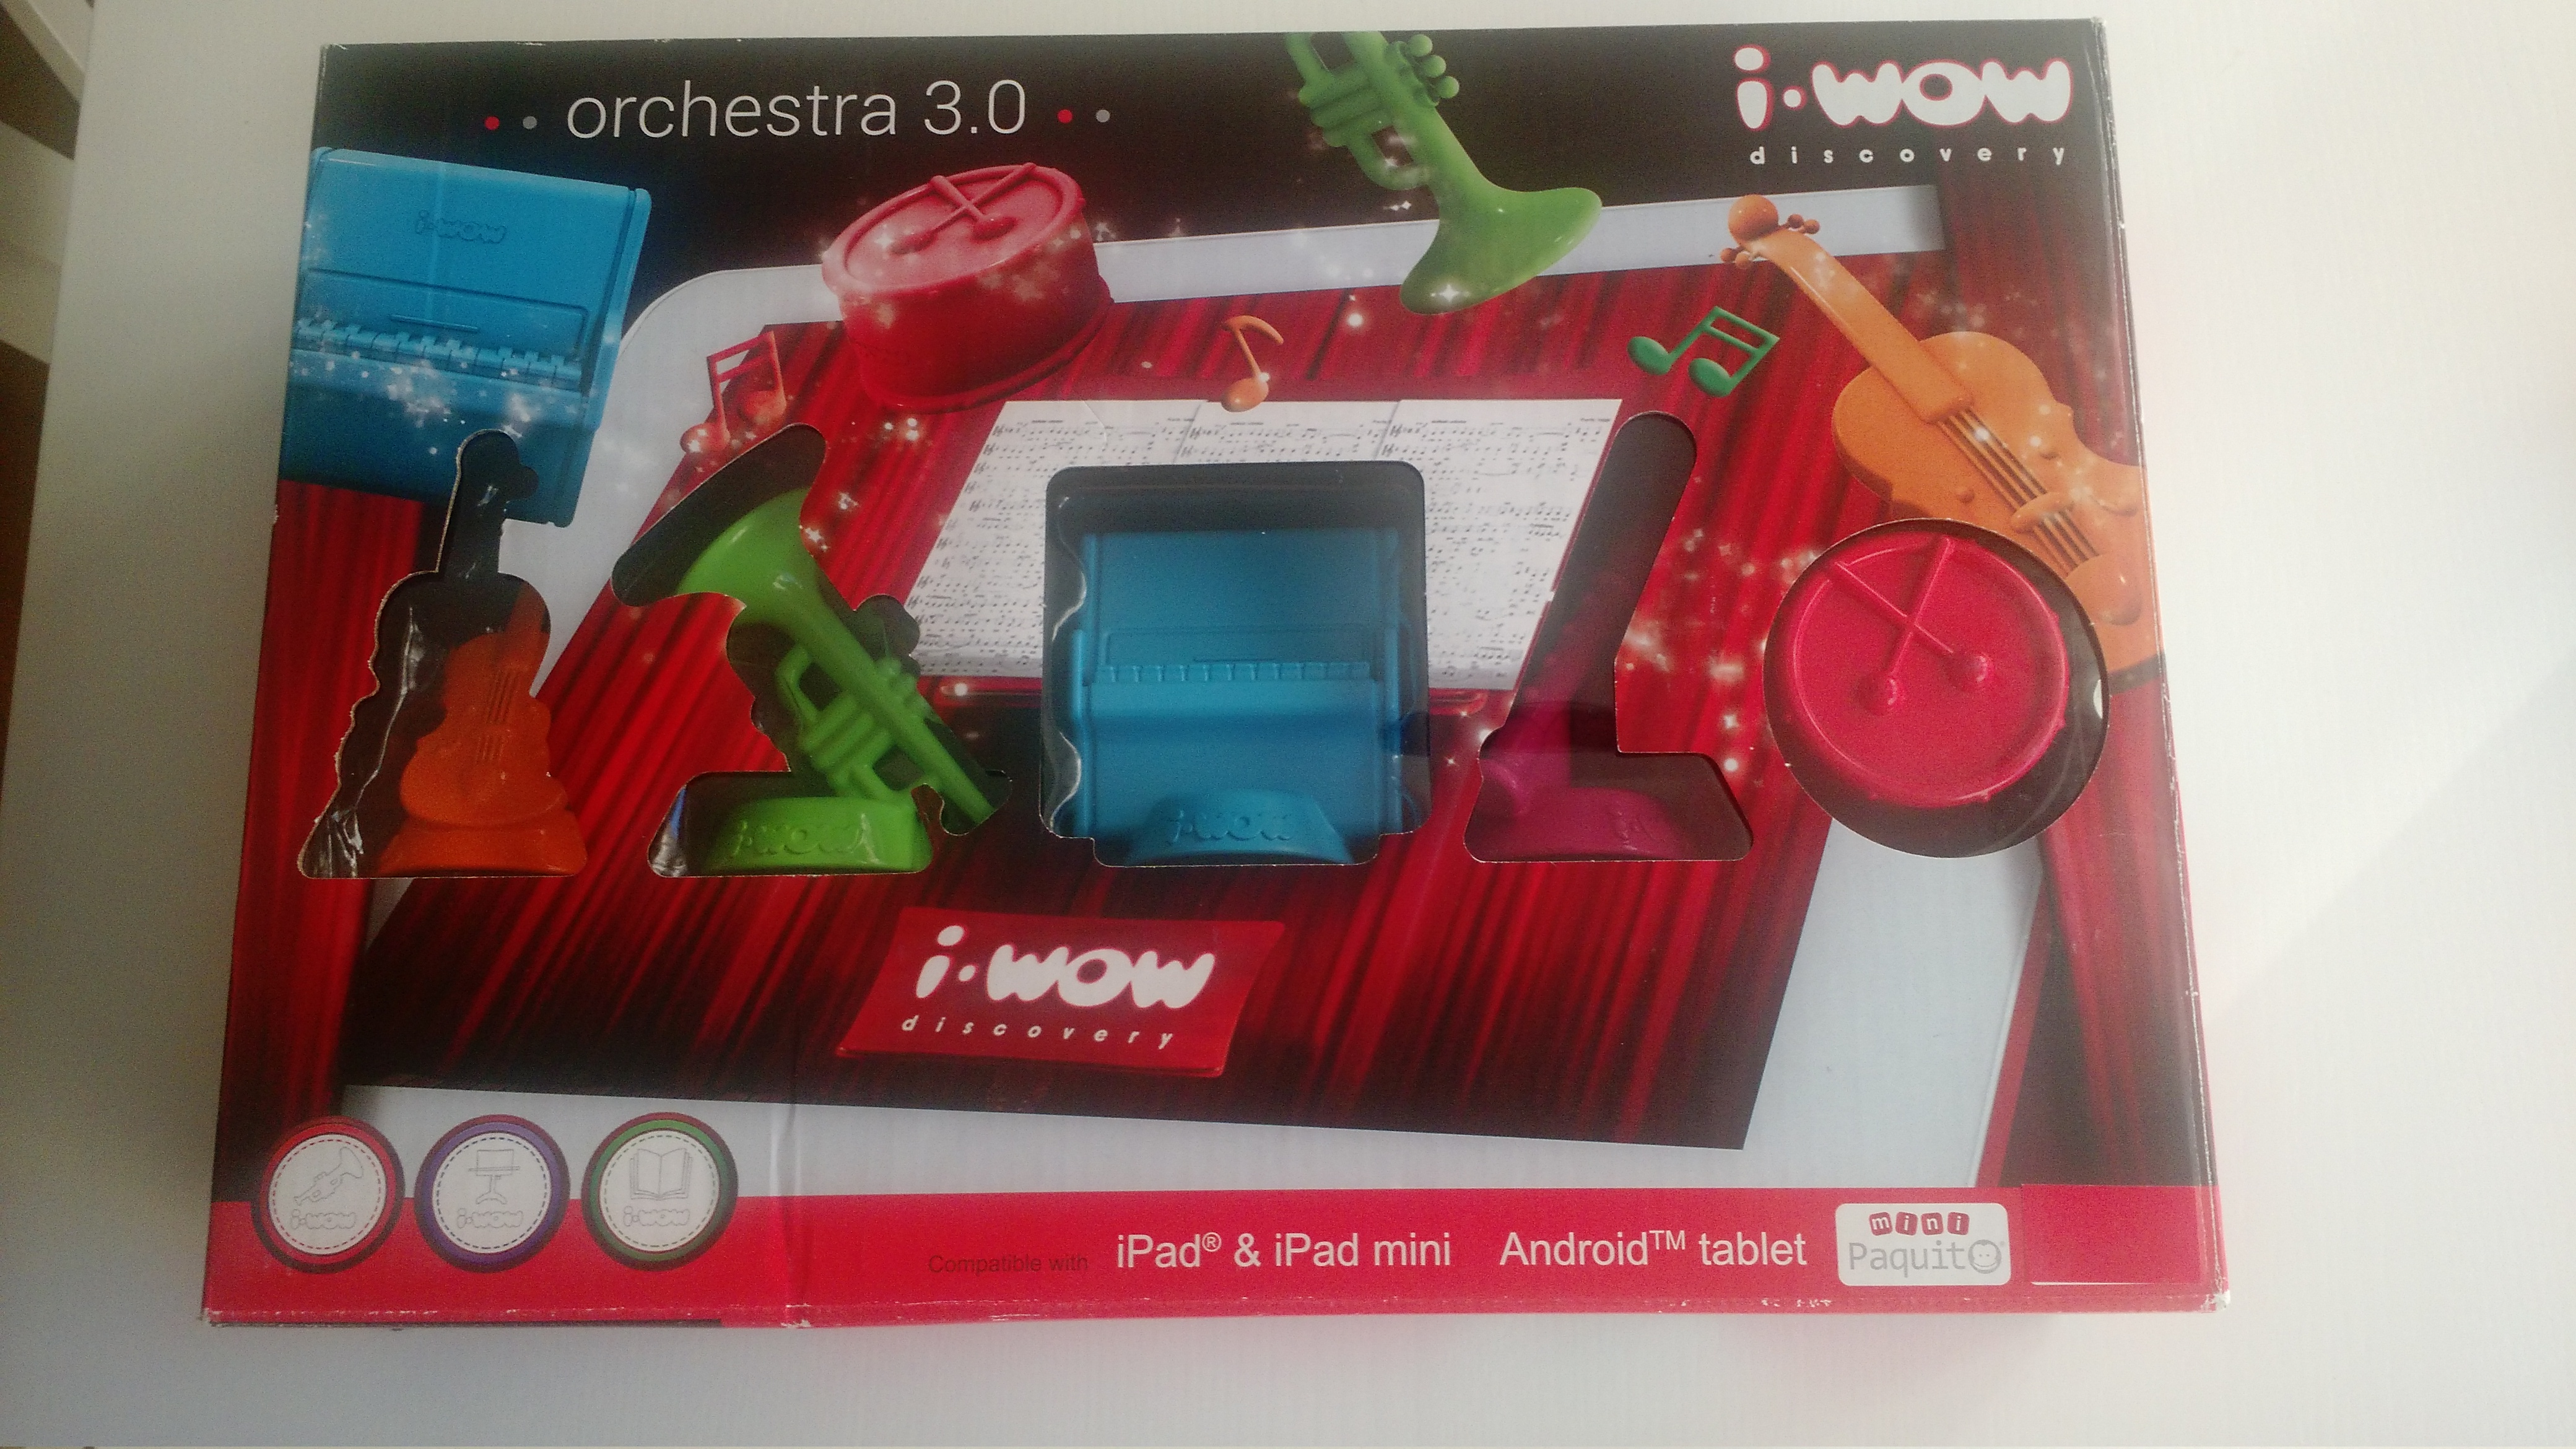
\includegraphics[width=350pt]{graphics/evaluation/instruments_pack.jpg}
\caption{Physical instrument pieces box}
\label{fig:instruments-pack}
\end{figure}

This will impact in the application user acquisition due to the fact that our target users will be the ones who have bought the physical game.

\FloatBarrier

We will study the acquisition metrics in two time periods. Firstly, we will look at the information obtained during the first year since the application was first released, this covers the period between August 2014 and August 2015. Then we will observe the information during the three years that the application has been available on the market which covers the period between August 2014 and February 2017.

\subsection{Number of users}

As we said, one of the most important metrics for user acquisition is the number of installations or the number of users which have download our application in their device.

In Figure \ref{fig:bars-first-year} we can see the new users engaged in the first year:

\begin{figure}[h]
\centering
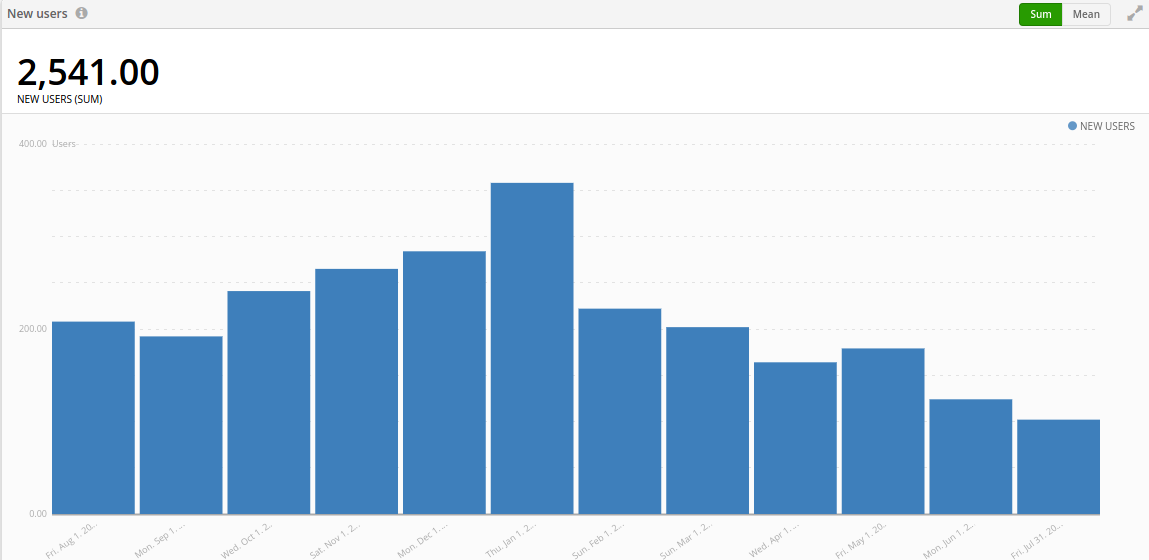
\includegraphics[width=350pt]{graphics/evaluation/bars_users_year.png}
\caption{New users in the first year from release}
\label{fig:bars-first-year}
\end{figure}

As wee can see, we got 2541 users in the first year. Every month the users increased an average of 200 new people. Also, we can observe that there is an evident increase of new users in the months of December and January, which is consequence of the increase of the physical packs sells within Christmas days.

In Figure \ref{fig:bars-all-year} we can see the new users obtained in the whole time our application have been on the market:

\begin{figure}[h]
\centering
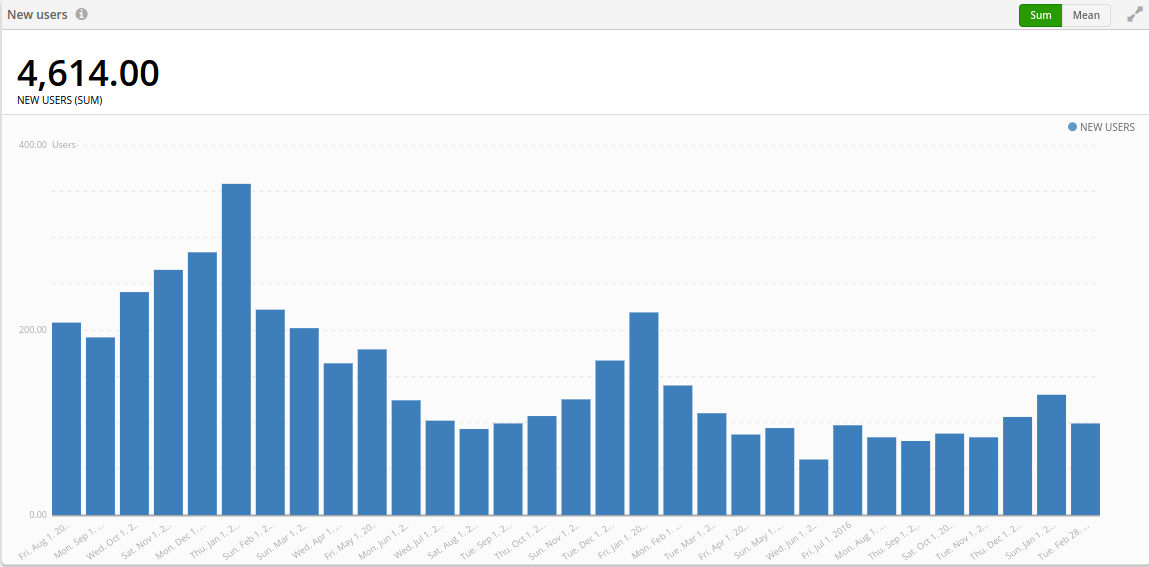
\includegraphics[width=350pt]{graphics/evaluation/bars_users_all.png}
\caption{New users since application first release}
\label{fig:bars-all-year}
\end{figure}

\FloatBarrier

As wee can see, we got 4641 users since our application first release. Also, we can observe that after first year new installations have been decreasing with the exception of the Christmas months described earlier. Even so, during 2016 our game has been constantly downloaded by an average of 100 new users.

\subsection{Users location}

Due to the physical instrument pack is sold in the countries list in the Table \ref{tab:countries}, is very useful to observe new user distribution across the world.

\begin{table}[!htpb]
\centering
    \begin{tabular}{|c|c|c|c|c|}
	\hline
	Argentina & Bulgaria & Colombia & Greece & Hungary \\
	\hline
	Israel & Latvia & Mexico & Poland & Qatar \\
	\hline
	Romania & Saudi Arabia & Switzerland & United Arab Emirates & Uruguay \\
	\hline
	Azerbaijan & China & France & Holland & ~\\
	\hline
	Italy & Lithuania & Peru & Portugal & ~\\
	\hline
	Russia & Spain & Turkey & United States & ~\\
    \hline
    \end{tabular}
\caption{Countries were the physical instrument pack is sold}
\label{tab:countries}
\end{table}

\FloatBarrier

In Figure \ref{fig:map-first-year} we can see the world distribution map of users engaged in the first year:

\begin{figure}[h]
\centering
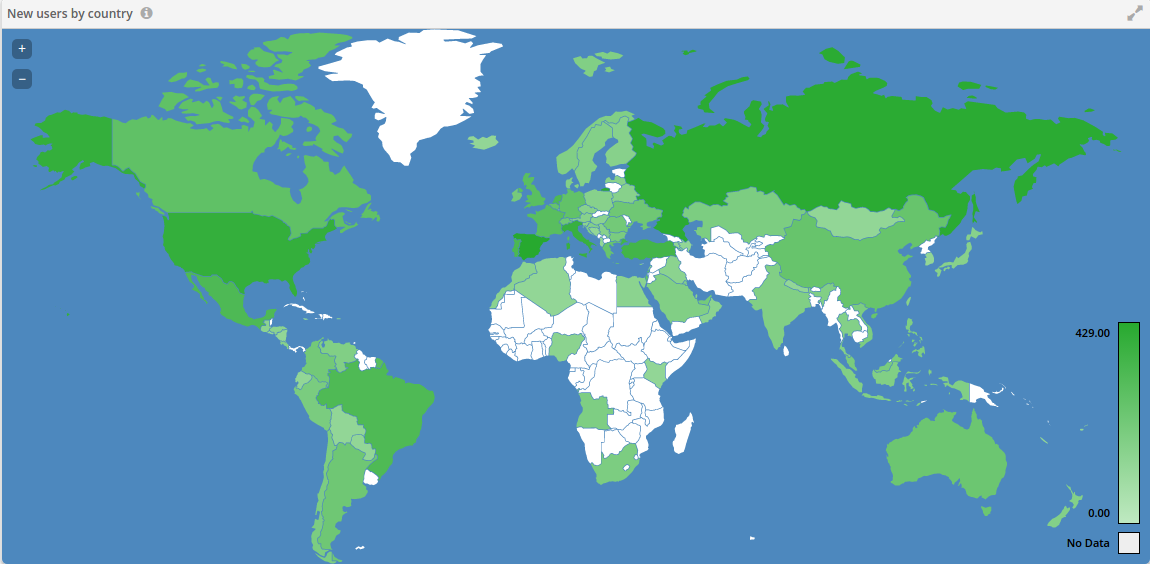
\includegraphics[width=350pt]{graphics/evaluation/map_users_year.png}
\caption{New users location in the first year from release}
\label{fig:map-first-year}
\end{figure}

Also, in Figure \ref{fig:chart-first-year} we can observe the top four countries where the game have been downloaded within this period:

\begin{figure}[h]
\centering
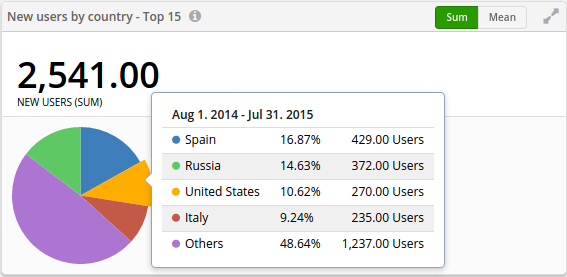
\includegraphics[width=200pt]{graphics/evaluation/chart_users_year.png}
\caption{New users location in the first year from release top countries}
\label{fig:chart-first-year}
\end{figure}

\FloatBarrier

As we can see, the application have been installed from most of the countries located in Europe and America, as long as many countries located in Asia. Also, Spain, Russia, USA and Italy are the countries where most of the users came from.

In Figure \ref{fig:map-all-year} we can see the world distribution map of users obtained in the whole time our application have been on the market:

\begin{figure}[h]
\centering
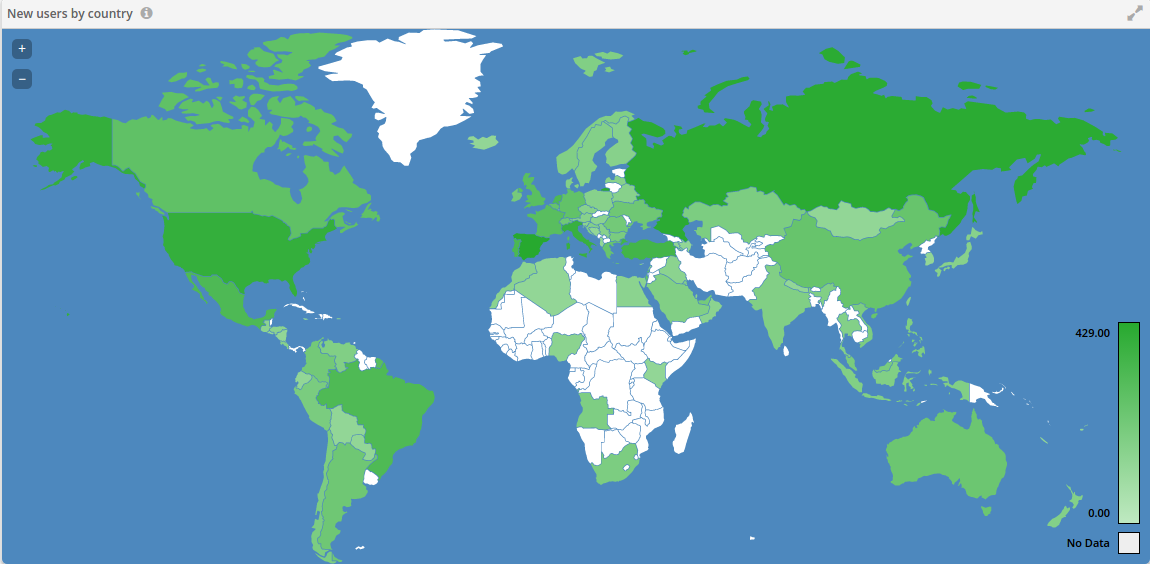
\includegraphics[width=350pt]{graphics/evaluation/map_users_year.png}
\caption{New users location since application first release}
\label{fig:map-all-year}
\end{figure}

Also, in Figure \ref{fig:chart-all-year} we can observe the top four countries where the game have been downloaded within this period:

\begin{figure}[h]
\centering
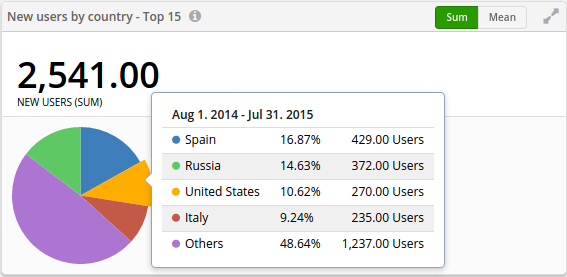
\includegraphics[width=200pt]{graphics/evaluation/chart_users_year.png}
\caption{New users location since application first release top countries}
\label{fig:chart-all-year}
\end{figure}

\FloatBarrier

As we can see, the application have been installed from a few more countries from the ones in the first year. Also, Spain, Russia, USA and Italy are the countries where most of the users came from.

\section{Engagement}

\section{Quality}
